\chapter{视觉表达}
短文本对话希望根据一段短文字,计算机模仿人类给出连贯的有意义的回复。人类在对一段文字进行回复的时候会经历:理解问题——大脑思考——给出回答,这样的一个过程。但是怎么判断别人(或者计算机)是否真正理解了你的意思?这个问题似乎很难回答。在目前自然语言理解领域上,对其有两个定义,一个是基于行为的,一个是基于表示的。对于前者,如果你说“给我拿一杯茶来”,别人(机器人)真的按你说的做了(行为),就认为他了解了你的意思;而对于后者,如果你说“猴子爬树”,别人把它联系到了大脑中猴子爬树的概念(表示),就认为他理解了你的意思。

%(如图\ref{fig:robot_tea})

十几年前,脑科学研究中有一个有趣的发现。当把电极插到猴子的大脑前运动皮质(pre-motor cortex)时,有一个脑细胞会在猴子自己吃香蕉和看别人吃香蕉时,同样处于兴奋状态,也就是说对猴子来说这个脑细胞对应着“吃香蕉”的概念。(猴子和人的运动都是由小脑控制, 但大脑的前运动皮质也与运动有关。)后来对人脑做类似的实验,但使用功能磁共振。让人实际做和想象做各种动作,比如跑步和想象跑步,爬树和想象爬树。结果发现,对同一动作,实际做和想象做大脑的前运动皮质中发生反应的部位完全一致。现在一个得到广泛支持的理论认为,对于同一个概念,大脑用固定的脑细胞去记忆,人理解语言的过程,就是激活相关概念的脑细胞,并关联这些概念的过程表示同一个概念的脑细胞,可以通过不同的方式被激活。例如,有一个细胞表示人在喝水,当你看到人在喝水的时候,或者当你从书中读到人在喝水的时候,这个脑细胞同样会被激活。这也能解释为什么我们在读小说的时候常常有身临其境的感觉。

每个人把自己经历的事件进行编码,存储记忆在脑细胞中,在与外界的交互中这些脑细胞被激活,相关的记忆被唤醒。所以,不同人对同样的语言会有不同的理解,因为他们的经历不同。但也有许多共性,因为大家在交流过程中,相互激活对方脑中的表示相同内容的细胞。发明比喻的时候,大脑中表示两个不同概念的部位都开始兴奋,相关的脑细胞之间产生新的连接,概念之间产生关联,这个过程被称为神经结合(neural binding),是现在脑科学研究的重要课题\footnote{Lakoff G. What Studying the Brain Tells Us About Arts Education, 2013.}。

语言的理解实际上是一个非常复杂的过程,动用了各种各样的感官,动用了大脑中所有的相关知识。我们的研究想让计算机读到一个短文本的时候能模拟人读到它的时候大脑产生的概念。这个过程就像是一个刚刚渡过婴儿期开始定义这个世界的孩子,她一开始一定没有“树”概念,她是在见过许多现实中的树,照片中的树,图画中的树之后才有了“树”的概念。也就是说,这样的概念其实是来自于这个孩子的视觉感受,当她在产生“树”的概念时是这些视觉图像的浓缩。正如“树”在脑海中会浮现出一个“树”的图片,我们在看到一段短文本对其产生概念,会在脑海中产生视觉图像,当然这样的视觉图像并不是在所有的短文本上就会产生,比如“昧着良心”。因此我们认为,\textbf{当我们读到一段短文字,对其产生的概念是否能用图像表示定义为短文本的视觉表达}。
\begin{figure}[ht]
\centering
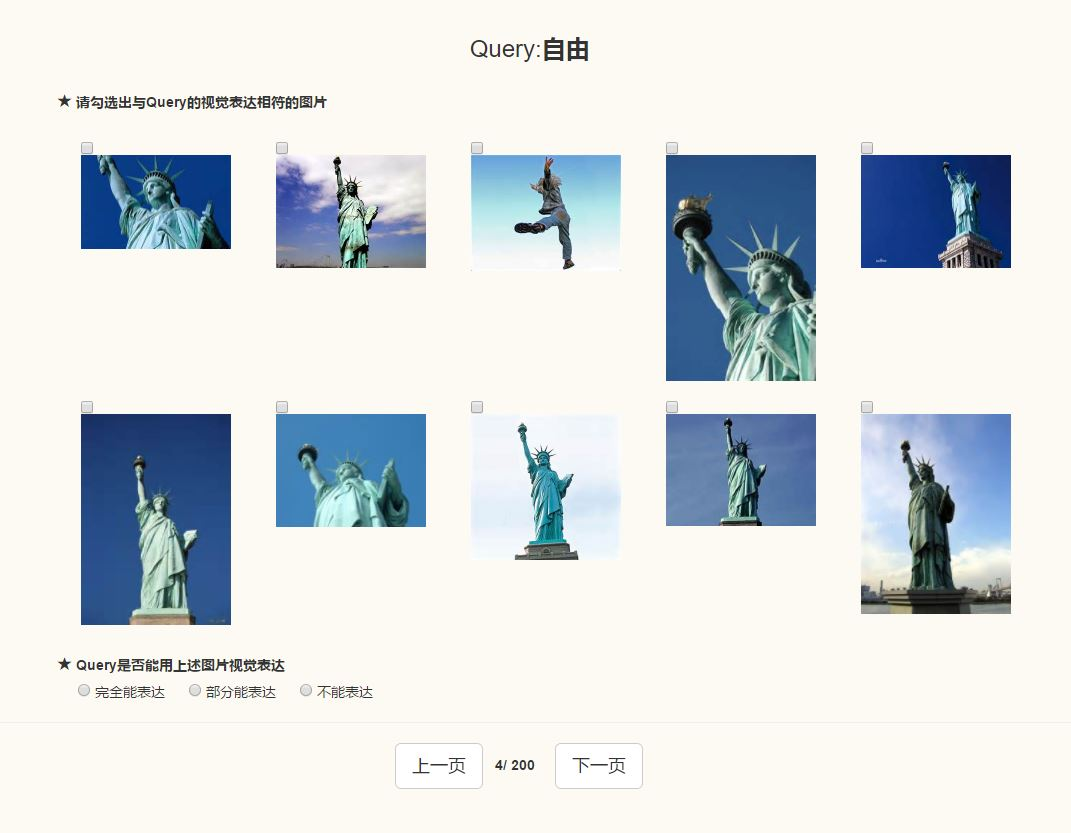
\includegraphics[width=14cm]{quest_vision}
\caption{图片视觉表达问卷调查} \label{fig:quest_vision}
\end{figure}
对于对话系统来说,它在看到一段短文本时,产生概念是什么?对于计算机来说。我们可以通过图片搜索引擎轻易地将短文本转化成图像集合。但是怎么判断这些图像集合能否等价于其视觉表达呢?我们将每个进行图片搜索的短文本称为一个查询用Query表示,将图片搜索得到的结果进行了人工标注如图\ref{fig:quest_vision}。标注员能够在一个页面里看到Query(查询)的短文本,和Query(查询)通过图片搜索得到的图片集合。标注员需要回答Query(查询)是否能用上述图片视觉表达以及勾选出符合标注员对短文本产生概念的视觉表达的图像。经过反复的人工标记,我们得到了以下准则:
\begin{itemize}
	\item     Query(查询)经过图片搜索得到的图片能够与其查询的短文本在人脑海中联系的的视觉表达相关,视为图片能作为Query(查询)的视觉表达。
	\item  当Query(查询)经过图片搜索得到的图片能作为Query(查询)的视觉表达的数量足够多时,视为与Query的意思能用图片视觉表达,数量不够的时候视为Query的意思能用上述图片部分视觉表达
	\item   当搜索得到的图片集有多个相同的语义时,当短文本的语义存在多个时,以及当符合Query(查询)视觉表达的图片数量不够多时,都视为Query能用搜索得到的图片集部分视觉表达
	\item    当搜索得到的图片集数量不足,或者图片杂乱无章时,视为Query(查询)不能用图片视觉表达。
\end{itemize}

在反复标记的过程中我们发现很多有趣的东西。除了我们很容易联想到的一些生活中的物品比如笔,树有视觉表达,在图\ref{fig:quest_vision}中,我们定义的一些在现实中没有的虚无的东西,也找了一致表达。在这个例子中图片搜索引擎返回给我们了很多自由女神像的图片,这跟我们人类的常识相符,我们使用自由女神像来代表自由,这是我们想要的在文字之外的关联。在另一个层面说,我们想要通过搜索引擎来寻找短文本一致的视觉表达。我们认为如果一个Query(查询)返回的图片越多一致的图片,这个图片是其人在脑海中的视觉表达概率越高。

另一个有意思的例子是Query:“玉米”的消费力,这样的一个Query(查询)在图片搜索后得到的结果是李宇春演唱会的图片。“玉米”除了是我们知道的食物之外,还是李宇春粉丝团的名字。在经过图片搜索引擎视觉表达后,像是经过了一轮人的思考和联系之后得到的视觉表达。同样的例子还出现在,在对帖子进行视觉表达后聚类中,关于食物话题的帖子的视觉表达会聚类在一起。我们认为经过图像表达可以比文字更能表示贴近我们脑海中的形象。

为了区别于Post(帖子),我们特意使用了Query(查询)来表示用于图片搜索的短文本。在本文的研究中,我们为了使Post(帖子)能够更好的进行图像表达,后续的相关章节会讨论关于帖子怎么变成Query(查询)。

在我们想设计的对话系统想要模拟人在理解短文本过程中是否利用到了我们的视觉感官系统。我们通过将短文本(帖子)变成一些相关的Query(查询),将Query(查询)得到图片集定义为计算机能够理解的短文本的视觉表达。

\subsection{图片搜索引擎}
由于搜索引擎已经花费了大量精力来完善他们官方使用的图像检索服务,我们可以很轻易收集标签图像。我们可以通过搜索图像标题、文件名和周围文本等方式来检索图像。现在各大图片搜索引擎都提供了搜索图片的API,要实现自动检索图像,我们可以将一个单词或短语(本文我们统一称为Query查询)作为HTTP查询提供给搜索引擎,并直接下载所返回的均匀缩略图,而不是直接下载原图像。一个是因为源网站图像要返回源网站下载,所以不如缩略图稳定;二是最后可能涉及的查询Query数量很多,考虑到存储空间;三是为图像大小相对均匀,这样在提取特征和问卷调查时候需要考虑图片差别。

各大图片搜索引擎提供的自动检索的接口都设置了流量限制,而我们的研究和对话系统数量较大,我们的研究经费难以承担。在宋睿华老师的帮助下,我们的难题得到了解决。因此本文的研究都使用Bing的图像搜索(https://www.bing.com/images)作为搜索引擎。我们的自动检索接口检索所得图片和人工检索结果一致。

\subsection{图片集数量}
我们希望通过图片搜索后的图片的集合来代表Query查询的图像表达。但是,显然我们不能将所有的图片缩略图都下载下来。一个是程序运行时间和存储限制,第二个是人工标记也不能顾上。我们当然希望能用最少的图片集数量来判断一个查询是否能够用视觉代表。
因此我们测试帖子进行分词后将帖子所有可能长度进行了分割。也是说,如果一个帖子有N个单词,我们可以将帖子分成N*(N-1)/2个Query(查询)。因此,现在的查询集合包含了所有可能长度。我们将图片搜索引擎的返回图片数量设置到30,记录每条Query查询的返回图片数量。100个测试帖子共分成了6,885个Query(查询),查询的最大词数是58,最小词数为1。返回图片数量如下图\ref{fig:ImageNum_Test_count}、\ref{fig:ImageNum_Test}所示,图片数量集中在最小值0和最大值30,在图片数量在10附件可以涵盖大部分Query查询。为了尽可能少的下载图片数量,本文中搜索引擎中一个Query查询取回的图片最大数量为10。





